\section{Zeitplanerstellung und Heuristiken} \label{sec:Heuristiken}

Um Zeitpläne für das \ac{mrcpsp} zu erstellen, gilt es die zugehörigen Constraints aus Abschnitt \ref{sec:MRCPSP} einzuhalten. Hierfür ist im Konzeptüberblick die Komponente \lstinline|Scheduler| vorgesehen. Des Weiteren müssen Lösungsansätze und Verfahren zur Lösung von Unsicherheiten auf eine gemeinsame Datenbasis verglichen werden, um für diese Zeitpläne erstellen zu können. Hierfür sind \lstinline|Benchmark Loader| und \lstinline|Benchmark Instance Sets| aus dem Abschnitt \ref{sec:Konzeptüberblick} vorgesehen. 

\subsection{Benchmarkinstanzen}

Zum Laden der Projektinstanzen von der PSPLIB ist ein \lstinline|BenchmarkLoaderService| implementiert, welcher anhand der Datenendung einen passenden Loader selektiert. Im Falle der PSPLIB für die Multi-Mode Projekterweiterung wird die Datenendung \lstinline|.mm| verwendet \cite[vgl.][S. 213 f.]{kolisch_psplib_1997}. Der vorgesehene \lstinline|BenchmarkPSPLIBMultiModeLoader| lädt aus der PSPLIB die vorgesehenen Struktur das Projekt einschließlich Metadaten, Aktivitäten, Aktivitätsbeziehungen, Modi und die Ressourcenanforderungen aus und überträgt diese innerhalb der im MRCPSP Framework vorgesehenen \acp{POJO}. Die einzelnen \acp{POJO} orientieren sich hierbei an den Subjekten und deren Beziehungen von der \ac{mrcpsp}-Problembeschreibung aus Abschnitt \ref{subsec:MRCPSP_MM}. Abbildung \ref{img:mrcpsp_framework_benchmarkloader} zeigt die Klassen des Benchmark Loaders und die der \acp{POJO} in einem UML-Klassendiagramm auf.

\subsection{Zeitplanerstellung}

Für die Erstellungen von \ac{mrcpsp}-Zeitplänen können unterschiedliche Repräsen-tationsformen verwendet werden. Neben den Aktivitäts- und Moduslisten existiert die Random Key Representation, welche in den Publikationen von \cite{sebt_efficient_2015} und \cite{kolisch_heuristic_1998} verwendet wird. Diese Arbeit beschränkt sich jedoch nur auf die Aktivitäts- und Moduslisten, welche in den Abschnitten \ref{subsec:SGS_Aktivitaeten} und \ref{subsec:SGS_Modi} eingeführt wurden. Hierfür ist eine Klasse \lstinline|ActivityListRepresentation| vorgesehen, die von der Klasse \lstinline|ScheduleRepresentation| erbt und zwei Felder für die Aktivitäten und für die Modi vorsieht. Diese Repräsentationsform wird von den (Meta-)Heuristiken zur Erstellung von Schedules genutzt. Abbildung \ref{img:mrcpsp_framework_schedulerheuristiken} stellt das UML-Klassendiagramm für die Realisierung der Repräsentationsform, aber auch der Zeitplanerstellung und Heuristiken dar. \\

Der \lstinline|SchedulerService| erzeugt mit der Methode \lstinline|createSchedule(...)| Zeitpläne anhand von Aktivitäten- und Modirepräsentationen $I = (\lambda, \mu)$ gemäß des \ac{ssgs}. Hierbei werden die Ressourcenbelegungen über Intervalle (\lstinline|Interval|) festgehalten. Listing \ref{lst:scheduler_forward} zeigt den Algorithmus für das sequenzielle Abarbeiten der Aktivitäten und den zugehörigen Modi (\lstinline|ActivityMode|) auf. Für jeden \lstinline|ActivityMode| wird ein identischer Intervall auf alle zu verwendenden erneuerbaren Ressourcen erzeugt. Intervalle geben an, wie lange eine erneuerbare Ressource mit wie vielen Einheiten belegt ist. Sei $I$ ein Intervall mit $I = [a, b]$, dann ist $a$ die Startzeit und $b$ die Endzeit einer Aktivität mit Bezug auf die ausgewählte Modusdauer. Im Algorithmus wird $a$ mit \lstinline|potentialLowerBound| und $b$ mit \lstinline|potentialUpperBound| gesetzt. Es gilt, dass eine Aktivität erst gestartet werden kann, wenn alle Vorgänger komplett durchlaufen wurden (vgl. Abschnitt \ref{subsec:MRCPSP_RCPSP}). Zudem müssen Aktivitäten ohne Unterbrechungen mit der Menge an benötigten Ressourcen ausgeführt werden (vgl. Abschnitt \ref{subsec:MRCPSP_RCPSP}). \\

Im Algorithmus wird zunächst die initiale Startzeit \lstinline|potentialLowerBound| gemäß der Vorgängerbeziehungen selektiert. Es gilt zu überprüfen, ob für die Aktivität zum Zeitpunkt ausreichend Ressourcen vorliegen. Hierfür wird eine Schleife durchlaufen, die für jede Ressourcenart gemäß der (Modus-)Ressourcenanforderungen überprüft werden, ob diese in benötigter Zahl $r_{j,m,k} \land c_{j,m,l}$ vorliegen (vgl. Listing \ref{lst:scheduler_computeAvailableResourcesOnInterval}). Wenn dies der Fall ist, wird die Schleife mittels \lstinline|solutionFound = true| verlassen und das gefundene Intervall für alle relevanten Ressourcenarten im Zeitplan hinzugefügt. Wenn bei einer erneuerbaren Ressourcenart die benötigte Anzahl nicht vorliegt, wird ein neues Interval erzeugt, indem \lstinline|potentialLowerBound| und \lstinline|potentialUpperBound| um eins inkrementiert werden. Anschließend wird das neue Intervall erneut für alle benötigten Ressourcenarten überprüft. Diese Prozedur wird solange ausgeführt, bis ein geeignetes Intervall gefunden wurde. Sofern die Anzahl an benötigten erneuerbaren Ressourcen die generelle Verfügbarkeit überschreitet oder wenn bereits alle nicht-erneuerbaren Ressourcen verbraucht wurden, handelt es sich um einen ungültigen Plan und somit wird der Algorithmus über das Exception-Handling abgebrochen. Bei Durchlaufen aller Einträge der Aktivitäts- und Moduslisten entsteht somit für die Repräsentation $I = (\lambda, \mu)$ ein minimaler Zeitplan. \\

Über einen Zeitplan können jegliche Metriken berechnet werden. Hierfür ist eine abstrakte Klasse \lstinline|Metric<?>| vorgesehen. Diese wird von den konkreten Metriken geerbt. Die relevanteste Metrik stellt die Makespan dar, welche sich über die höchste Endzeit aller ermittelten Intervalle ableiten lässt. Weitere Metriken können die Robustheitsmessungen darstellen. Diese wiederum nutzen meist den freien Puffer von Aktivitäten, welche sich über das Backward Recursive Procedure berechnen lassen (vgl. Abschnitt \ref{subsec:Praediktive_Methoden}). \\ 

Während beim gewöhnlichen Forward Recursive Procedure die frühstmöglichen Start- und Endzeitpunkte gemäß der Aktivitäts- und Modusliste bestimmt werden, wird beim Backward Recursive Procedure eine Aktivität zum spätestmöglichen Zeitpunkt geschedulded \cite[vgl][S. 181]{al-fawzan_bi-objective_2005}. Somit ist es möglich, die spätesten Start- und Endzeitpunkte von Aktivitäten zu bestimmen, um so den Puffer einer Aktivität berechnen zu können \cite[vgl][S. 181]{al-fawzan_bi-objective_2005}. Dieser Algorithmus wird ebenfalls im \lstinline|SchedulerService| über die Methode \lstinline|createScheduleBackward()| realisiert.

\subsection{Heuristiken}
Eine Möglichkeit Aktivitäts- und Moduslisten $I = (\lambda, \mu)$ zu erzeugen, stellen zunächst die Heuristiken dar. Diese werden innerhalb der Arbeit verwendet, um initiale Zeitpläne für die Metaheuristiken zu erzeugen. Als Heuristiken werden die prioritäts-basierten Regeln für Aktivitäten (gemäß Tabelle \ref{tab:ActivityRules}) und die Selektionsregeln für Modi (gemäß Tabelle \ref{tab:ModeRules}) über den \ac{ssgs} eingesetzt. \\

Die zu implementierenden Prioritätsregeln erben von der Klasse \lstinline|ActivityHeuristic|, die eine abstrakte Methode \lstinline|determineActivityPriorityValue(...)| besitzt. Die konkretisierende Klasse implementiert die Methode anhand der Prioritätsregel und gibt den Prioritätswert für eine Aktivität \lstinline|Activity| zurück. Innerhalb der Abbildung \ref{img:mrcpsp_framework_schedulerheuristiken} lassen sich somit die konkreten Klassen aus Tabelle \ref{tab:ActivityRules} einschließlich einer Zufallsregel erkennen:
\begin{itemize}
    \item \lstinline|GRPWHeuristic|
    \item \lstinline|LFTHeuristic|
    \item \lstinline|LSTHeuristic|
    \item \lstinline|MSLKHeuristic|
    \item \lstinline|MTSHeuristic|
    \item \lstinline|RandomActivityHeuristic|
\end{itemize}
Das Prinzip gilt ebenfalls für die zu implementierenden Selektionsregeln, welche die Klasse \lstinline|ModeHeuristic| vorsieht. Über die Methode  \lstinline|determineModePriorityValue(...)| wird der Selektionswert für eine Aktivität mit einem bestimmten Modus berechnet. Abbildung \ref{img:mrcpsp_framework_schedulerheuristiken} zeigt die konkreten Klassen für die implementierten Selektionsregeln einschließlich einer Zufallsregel auf: 
\begin{itemize}
    \item \lstinline|LPSRDHeuristic|
    \item \lstinline|LRSHeuristic|
    \item \lstinline|LTRUHeuristic|
    \item \lstinline|SMFHeuristic|
    \item \lstinline|RandomModeHeuristic|
\end{itemize}
\lstinline|Heuristic| sieht jeweils eine konkrete \lstinline|ActivityHeuristic| und \lstinline|ModeHeuristic| vor und er-möglicht somit etwaige Kombinationen zwischen den Regeln. Dreh und Angelpunkt für die Erzeugung von heuristischen Lösungen stellt der \lstinline|HeuristicDirector|. Die Methode \lstinline|constructScheduleRepresentation(...)| erzeugt anhand eines Objektes der Klasse \lstinline|Heuristic| und einer Angabe des Sampling-Verfahrens entsprechende Instanzen vom Typ \lstinline|ScheduleRepresentation|, welche konkret die Aktivitäts- und Moduslistenrepräsentation darstellen. Dies geschieht, indem Aktivitäten und Modi gemäß des \ac{ssgs} von Abschnitt \ref{subsec:SGS} sequenziell selektiert werden. Beim Sampling stehen die folgenden Möglichkeiten zur Verfügung:

\begin{description}
\item[Single] Aktivitäten und Modi werden gemäß ihres Prioritäts- bzw. des Selektionswertes selektiert. Zunächst wird in einer Phase $g$ für alle möglichen Aktivitäten $\mathcal{D}_g$ jeweils ein Modus gemäß des besten Selektionswertes $s(j, m) \, \forall j \in \mathcal{D}_g$ ausgewählt. Im Anschluss wird die Aktivität einschließlich des selektierten Modus über den Prioritätswert $v(j)$ selektiert. 
\item[\acf{RBRS}] Aktivitäten und Modi gilt es ebenfalls über den Prioritäts- bzw. Selektionswert auszuwählen, jedoch werden hierfür Wahrscheinlichkeiten vorgesehen, um so abweichend mehrere Lösungen zu erhalten. Das Prinzip von \ac{RBRS} als Multi-Pass Sampling Methode wurde bereits im Abschnitt \ref{subsec:SGS_RBBRS} erläutert. Der Parameter $\epsilon$ wird dem Wert $\epsilon = \max(0.001, \min_{i \in \mathcal{D}_g} v(i))$ zugewiesen, welche die Empfehlung von Drexl (1991) gemäß \cite[][S. 7]{kolisch_heuristic_1998} dahingehend modifiziert, sodass Epsilon nie null ist. Dies verhindert invalide Divisionen. Für den Parameter $\alpha$ wird empirisch der konstante Wert $\alpha = 10$ festgelegt. Insbesondere bei Benchmarks mit hohem nicht-erneuerbarem Ressourcenverbrauch und einer hohen Anzahl an Aktivitäten können mithilfe der Selektionsregel \lstinline|LRSHeuristic| mit hoher Wahrscheinlichkeit zunächst gültige Zeitpläne erstellt werden, da die noch benötigten nicht-erneuerbaren Ressourcen in Relation zu den verfügbaren nicht-erneuerbaren Ressourcen gestellt werden. Es wird der Modus ausgewählt, für welcher in Relation die meisten Ressourcen vorhanden sind. Insbesondere diese Selektionsregel profitiert von einem hohen $\alpha$-Parameter, um so eher stärker an der Regel orientierte Lösungen zu erhalten, aber trotzdem gewisse Abweichungen zu erlauben. 
\end{description}

\subsection{Visualisierung}

Innerhalb der Anwendung werden Konsolenausgaben genutzt, um so den Fortschritt und die Ergebnisse der Experimente auszugeben. Nach Durchlaufen eines Lösungs-ansatzes wird der beste Zeitplan einschließlich der Aktivitäts- und Modusliste, Makespan und ggf. der Robustheitsmetrik ausgegeben. Dadurch können Zeitpläne reproduziert werden. Hierfür wird beim Initialisieren des MRCPSP-Frameworks ein Thread erzeugt, welcher parallel zu den Berechnungen läuft. Dieser wird über den Service \lstinline|CommandLineToolService| implementiert und nimmt den Benchmarknamen, die Aktivitätsliste und die Modusliste einzeln entgegen und erstellt über den Scheduler einen manuellen Zeitplan. Dieser wird sowohl in Textform als auch grafisch visualisiert. \\

Viele Teilbereiche dieser Arbeit werden über Zahlen verdeutlicht. Um jedoch ein Bild von erstellten Zeitplänen machen zu können eignet sich die Möglichkeit der grafischen Visualisierung. Hierfür ist der \lstinline|VisualizationService| vorgesehen, welcher den Projektplan eines Benchmarks, aber auch zugehörige Zeitpläne über die Ressourcenbelegungen grafisch darstellen kann.

\begin{figure}[H]
    \centering
    \noindent\makebox[\textwidth]{%
    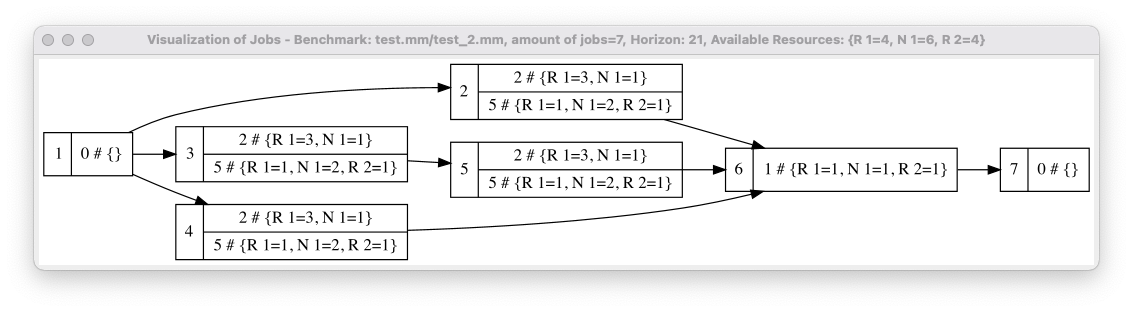
\includegraphics[width=\textwidth]{assets/img/04_Umsetzung/ScreenshotPlan.png}
    }
    \caption{Screenshot einer Projektplan-Visualisierung} 
    \label{img:visualization_projectplan}
    \source{Eigene Darstellung}
\end{figure}

Abbildung \ref{img:visualization_projectplan} stellt einen Screenshot von der Visualisierung eines beispielhaften \ac{mrcpsp}-Projektplans über den \lstinline|VisualizationService| dar. Die Darstellungsweise wurde bereits im Abschnitt \ref{subsec:MRCPSP_MM} erläutert. Für die Generierung von Projektplänen wird die Software Graphviz von \cite{att_graphviz_2021} verwendet. \lstinline|visualizeBenchmark(benchmark)| visualisiert einen Projektplan, indem jede Aktivität einen Knoten repräsentiert und diese gemäß ihrer Nachfolgebeziehungen verbunden werden. Die Positionierung der Knoten erfolgt über Graphviz automatisch.  

\begin{figure}[H]
    \centering
    \subfloat[][]{
        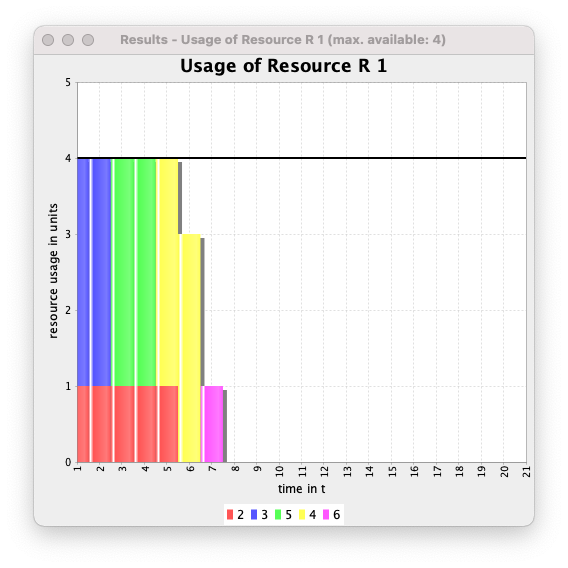
\includegraphics[width=0.51\linewidth]{assets/img/04_Umsetzung/ScreenshotR1.png}
        \label{img:visualization_schedule_a}
    }%
    \subfloat[][]{
        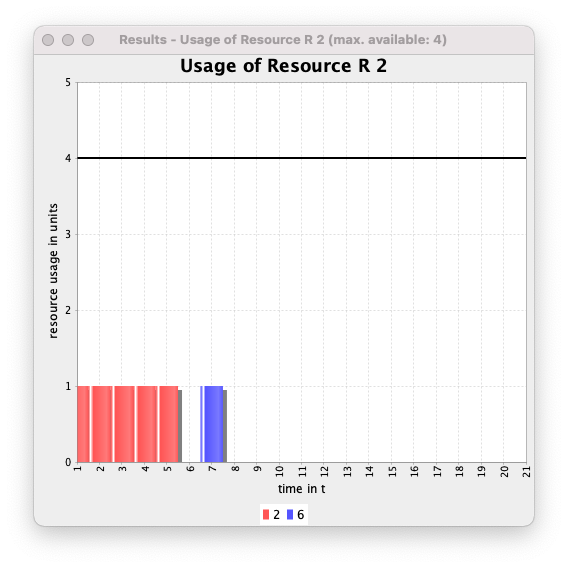
\includegraphics[width=0.51\linewidth]{assets/img/04_Umsetzung/ScreenshotR2.png}
        \label{img:visualization_schedule_b}
    }%
  
    \caption{Screenshots einer Zeitplan-Visualisierung über erneuerbare Ressourcenarten für den Projektplan aus Abbildung \ref{img:visualization_projectplan}} 
    \label{img:visualization_schedule}
    \source{Eigene Darstellung}
\end{figure}
Abbildung \ref{img:visualization_schedule} zeigt Screenshots für die Darstellung von Zeitplänen auf. Hierbei stellen Abb. \ref{img:visualization_schedule_a} und  Abb. \ref{img:visualization_schedule_b} den Ressourcenverbrauch für die erneuerbare Ressourcenart $R_1$ und $R_2$ dar. Die vertikalen Balken stellen den Ressourcenverbrauch von Aktivitäten dar, welche über die Farbe differenziert werden. Das maximale Ressourcenlimit für eine Ressource $R_k$ wird über die horizontale schwarze Linie angegeben. Folglich darf diese gemäß der \ac{mrcpsp}-Beschränkung aus Formel \ref{align:mrcpsp_constraint3} nicht überschritten werden. \\

Für den nicht-erneuerbaren Ressourcenverbrauch wird die gleiche Darstellung wie bei dem erneuerbaren Ressourcenverbrauch verwendet. Jedoch werden die nicht-erneuerbaren Ressourcen bis zum Ende des Zeitplans verwendet. Dies wird in Abbildung \ref{img:visualization_schedule_c} verdeutlicht. \\

Für die Visualisierung von Zeitplänen wird die Methode \lstinline|visualizeSchedule(schedule)| aus der Klasse \lstinline|VisualizationService| verwendet. Hierbei werden die \lstinline|XYPlot| aus der Bibliothek JFreeChart von \cite{gilbert_jfreechart_2021} verwendet, um die vertikalen Balken aufeinander stapeln zu können. 

\begin{figure}[H]
    \centering
    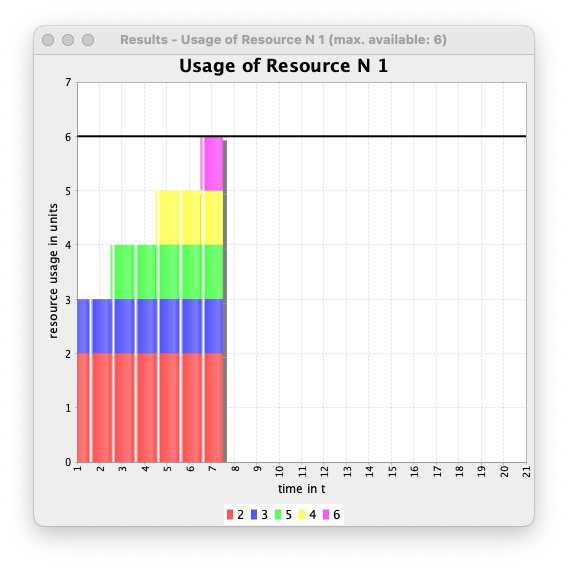
\includegraphics[width=0.47\linewidth]{assets/img/04_Umsetzung/ScreenshotN1.png}
    \caption{Screenshot einer Zeitplan-Visualisierung über nicht-erneuerbare Ressourcenarten für den Projektplan aus Abbildung \ref{img:visualization_projectplan}} 
    \label{img:visualization_schedule_c}
    \source{Eigene Darstellung}
\end{figure}